\section{Anwendungen}
\subsection{Digitalisierung}
\subsection{Auflösung}
Die A/D Auflösung in bit $n$ eines Sensor kann durch folgende Formel berechnet werden, falls Aufteilung linear ist:
\[
n = \lceil \log_2\left(\frac{\Delta}{a}\right) \rceil
\]
\textbf{Beispiel:}
$a = 1.0g$ und Messung von $0kg...20kg$ ergibt $15bit = \lceil \log_2\left(\frac{20000g}{1g}\right) \rceil$

\subsection{DGL von Model}
\todo{Tip: bei höchster Ableitung beginnen und dann schritt für schritt Gleichung aufstellen.}

\subsection{Zahnrad}
Dabei kann der Übersetzungsfaktor $n = \frac{Z2}{Z1}$ berechnet werden und Offset $O$ von entsprechendem Winkel hinzu addiert werden.
\begin{center}
	\begin{minipage}{0.35\textwidth}
		\begin{center}
			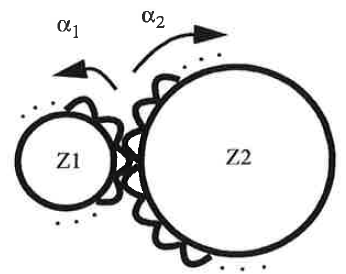
\includegraphics[width=0.25\linewidth,keepaspectratio=true]{Images/zahnrad_I}
			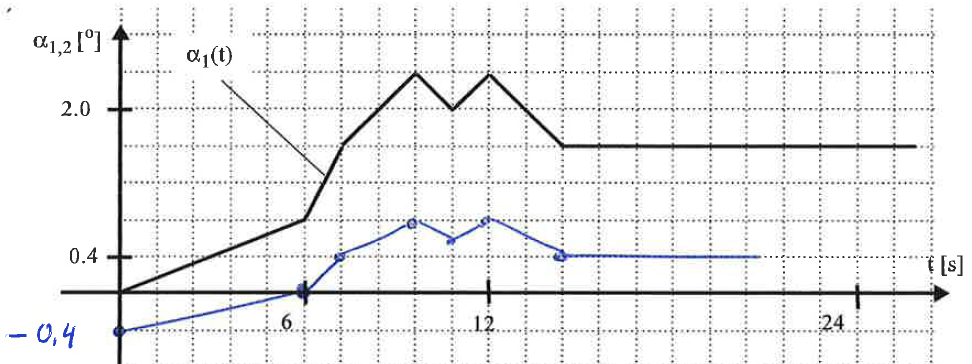
\includegraphics[width=0.5\linewidth,keepaspectratio=true]{Images/zahnrad_I1}
		\end{center}
	\end{minipage}%%% to prevent a space
	\begin{minipage}{0.15\textwidth}
		\begin{align*}
			\alpha_2 = \frac{\Delta \alpha_1}{n} + O
		\end{align*}
	\end{minipage}
\end{center}

\begin{center}
	\begin{minipage}{0.35\textwidth}
		\begin{center}
			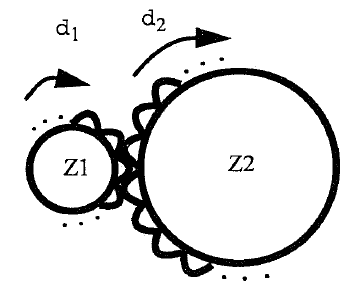
\includegraphics[width=0.25\linewidth,keepaspectratio=true]{Images/zahnrad_II}
			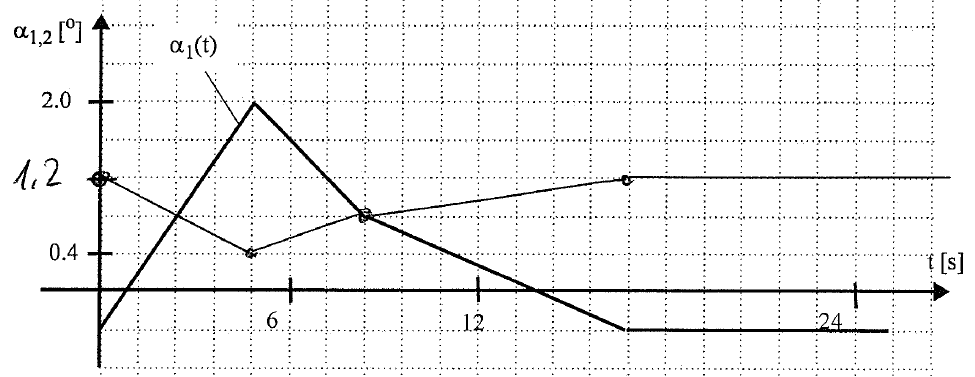
\includegraphics[width=0.5\linewidth,keepaspectratio=true]{Images/zahnrad_II2}
		\end{center}
	\end{minipage}%%% to prevent a space
	\begin{minipage}{0.15\textwidth}
		\begin{align*}
			\alpha_2 = -\frac{\Delta\alpha_1}{n} + O
		\end{align*}
	\end{minipage}
\end{center}

